\documentclass[12pt]{scrartcl}
\usepackage[sexy]{james}
\usepackage[noend]{algpseudocode}
\setlength{\marginparwidth}{2cm}
\usepackage{graphicx}
\usepackage{answers}
\usepackage{array}
\usepackage{tikz}
\newenvironment{allintypewriter}{\ttfamily}{\par}
\usepackage{listings}
\usepackage{xcolor}
\usetikzlibrary{arrows.meta}
\usepackage{color}
\usepackage{mathtools}
\newcommand{\U}{\mathcal{U}}
\newcommand{\E}{\mathbb{E}}
\usetikzlibrary{arrows}
\Newassociation{hint}{hintitem}{all-hints}
\renewcommand{\solutionextension}{out}
\renewenvironment{hintitem}[1]{\item[\bfseries #1.]}{}
\renewcommand{\O}{\mathcal{O}}
\declaretheorem[style=thmbluebox,name={Chinese Remainder Theorem}]{CRT}
\renewcommand{\theCRT}{\Alph{CRT}}
\setlength\parindent{0pt}
\usepackage{sansmath}
\usepackage{pgfplots}

\usetikzlibrary{automata}
\usetikzlibrary{positioning}  %                 ...positioning nodes
\usetikzlibrary{arrows}       %                 ...customizing arrows
\newcommand{\eqdef}{=\vcentcolon}
\newcommand{\tr}{{\rm tr\ }}
\newcommand{\im}{{\rm Im\ }}
\newcommand{\spann}{{\rm span\ }}
\newcommand{\Col}{{\rm Col\ }}
\newcommand{\Row}{{\rm Row\ }}
\newcommand{\dint}{\displaystyle\int}
\newcommand{\dt}{\ {\rm d }t}
\newcommand{\PP}{\mathbb{P}}
\newcommand{\horizontal}{\par\noindent\rule{\textwidth}{0.4pt}}
\usepackage[top=3cm,left=3cm,right=3cm,bottom=3cm]{geometry}
\newcommand{\mref}[3][red]{\hypersetup{linkcolor=#1}\cref{#2}{#3}\hypersetup{linkcolor=blue}}%<<<changed

\tikzset{node distance=4.5cm, % Minimum distance between two nodes. Change if necessary.
         every state/.style={ % Sets the properties for each state
           semithick,
           fill=cyan!40},
         initial text={},     % No label on start arrow
         double distance=4pt, % Adjust appearance of accept states
         every edge/.style={  % Sets the properties for each transition
         draw,
           ->,>=stealth',     % Makes edges directed with bold arrowheads
           auto,
           semithick}}


% Start of document.
\newcommand{\sep}{\hspace*{.5em}}

\pgfplotsset{compat=1.18}
\begin{document}
\title{MATH410: Homework 2}
\author{James Zhang\thanks{Email: \mailto{jzhang72@terpmail.umd.edu}}}
\date{\today}

\definecolor{dkgreen}{rgb}{0,0.6,0}
\definecolor{gray}{rgb}{0.5,0.5,0.5}
\definecolor{mauve}{rgb}{0.58,0,0.82}

\lstset{frame=tb,
  language=Java,
  aboveskip=3mm,
  belowskip=3mm,
  showstringspaces=false,
  columns=flexible,
  basicstyle={\small\ttfamily},
  numbers=left,
  numberstyle=\tiny\color{gray},
  keywordstyle=\color{blue},
  commentstyle=\color{dkgreen},
  stringstyle=\color{mauve},
  breaklines=true,
  breakatwhitespace=true,
  tabsize=3
}

\maketitle

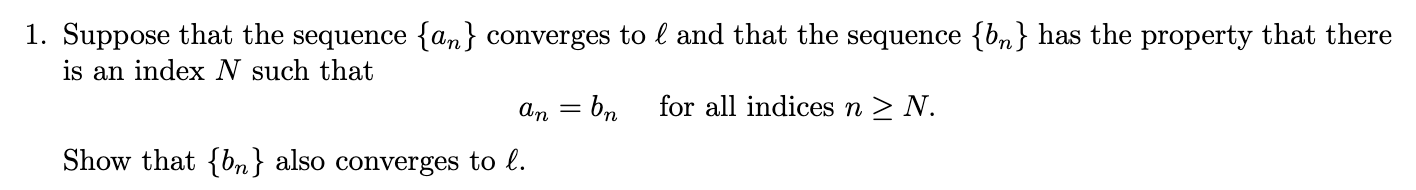
\includegraphics[width=15cm]{1.png}

Sketch: we want to show that $\{b_n\}$ converges to $l$. Therefore, we need to show the 
definition of convergence such that given an $\epsilon > 0$,  $|b_n - l| < \epsilon$ for all $n \geq N, N \in \NN$.

Let $\epsilon > 0$. By the definition of convergence, $\exists N_1 \ \in \NN$ such that 
\[|a_n - l| < \epsilon \ \forall \ n \geq N_1\]
Choose $N_2 = \max(N, N_1)$ where $N$ is the given index in the problem description and 
$N_1$ is the index that satisfies the definition of convergence given any positive $\epsilon$.

\begin{proof}
  By the definition of convergence, let $\epsilon > 0$ be given, and so $\exists \ N_1 \in \NN$ such that 
  \[|a_n - l| < \epsilon \ \forall \ n \geq N_1\]
  Let us choose $N_2 = \max(N, N_1)$. Since the above is true for all $n \geq N_1$, it must also 
  be true $n \geq \max(N, N_1)$. Therefore ,
  \[|a_n - l| < \epsilon \ \forall \ n \geq N_2\]
  Moreover, for all $n \geq N_2$, we know that $a_n = b_n$. By direct substitution into the absolute value, 
  \[|b_n - l| < \epsilon \ \forall \ n \geq N_2\]
  Thus, given any $\epsilon > 0$, there exists a threshold $N_2$ such that the definition of
  convergence is satisfied and so $\underset{n\to\infty}{\lim}b_n = l$ as desired.
\end{proof}

\newpage

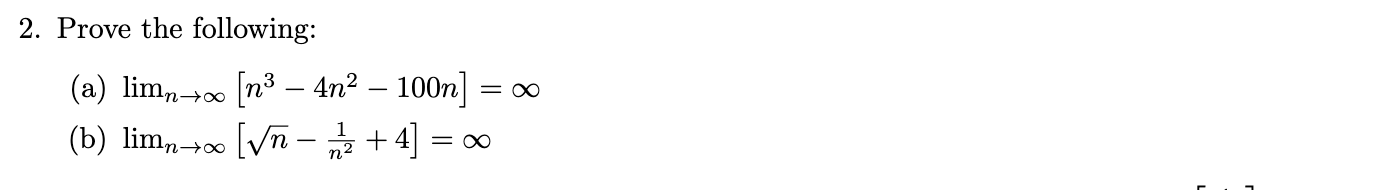
\includegraphics[width=15cm]{2.png}

\begin{enumerate}[a.]
  \item Sketch: we want to show that given some $M > 0$, $a_n > M \ \forall n \geq N, N \in \NN$.
  \[n^3 - 4n^2 - 100n > n^2 - 4n - 100 > n^2 - 15n - 100 = (n-20)(n+5) > M\]
  Choose $N > \max(M, 20)$.
  
  \begin{proof}
    Let $M > 0$ be given. By the Archimedian Principle, $\exists \ N \in \NN$ such that $N > \max(M, 20)$.
    
    Now observe the following operations 
    \[n^3 - 4n^2 - 100n > n^2 - 4n - 100\]
    where the right side of the inequality was obtained by dividing all terms by $n$. 
    \[n^2 - 4n - 100 > n^2 - 15n - 100 = (n-20)(n+5)\]
    which also must be true since $n > 0$, and the equality came by factoring. Now note that 
    $N > \max(M, 20)$ and $n \geq N$. Therefore, 
    \[(n-20)(n + 5) \geq (N-20)(N+5) > (M-20)(M + 5) > M\] 
    Thus, we have shown the definition of divergence because for any given $M > 0$, we can find a threshold $N$ such that
    \[n^3 - 4n^2 - 100n > M \ \forall \ n \geq N\]
    which implies that
    \[n^3 - 4n^2 - 100 \to \infty \text{ as } n \to \infty \implies \underset{n\to\infty}{\lim}n^3 - 4n^2 - 100n = \infty\]
  \end{proof}

  \item Sketch: we WTS to show that for $M > 0$, then $a_n > M \ \forall \ n \geq N, N \in \NN$.
  \[\sqrt{n} - \frac{1}{n^2} + 4 > \sqrt{n} - \frac{1}{n^2} \geq \sqrt{n} - \frac{1}{n} = (n^{\frac{1}{4}} + \frac{1}{\sqrt{n}})(n^{\frac{1}{4}} - \frac{1}{\sqrt{n}})\]
  Choose $N > \max(M^4$, 1).

  \begin{proof}
    Let $M > 0$ be given. By A.P., $\exists \ N \in \NN$ such that $N > \max(M^4, 1)$.
    Note that
    \[\sqrt{n} - \frac{1}{n^2} + 4 > \sqrt{n} - \frac{1}{n^2} \ \forall \ n\]
    Furthermore, note that $\frac{1}{n^2} \leq \frac{1}{n} \ \forall n$. Therefore, 
    $-\frac{1}{n^2} \geq -\frac{1}{n} \ \forall n$ as well, by mutliplying both sides by $-1$ 
    and subsequently reversing the direction of the inequality. Thus, 
    \[\sqrt{n} - \frac{1}{n^2} \geq \sqrt{n} - \frac{1}{n}\]
    Recall that $n \geq N$ and so 
    \[\sqrt{n} - \frac{1}{n} \geq \sqrt{N} - \frac{1}{N} = (N^{\frac{1}{4}} + \frac{1}{\sqrt{N}})(N^{\frac{1}{4}} - \frac{1}{\sqrt{N}})\]
    \[> (M + \frac{1}{M^2})(M - \frac{1}{M^2}) > M\]
    Note that this last inequality is always true, since we choose $N > \max(M^4, 1)$. Therefore, 
    the second term $(M - \frac{1}{M^2}) > 1$ for all of our choices of $n \geq N$. Thus, we've shown that 
    for any given $M > 0$, we can find a threshold $N$ such that 
    \[\sqrt{n} - \frac{1}{n^2} + 4 > M \ \forall \ n \implies \lim_{n\to\infty}\sqrt{n} - \frac{1}{n^2} + 4 = \infty\]
  
  \end{proof}

\end{enumerate}

\newpage

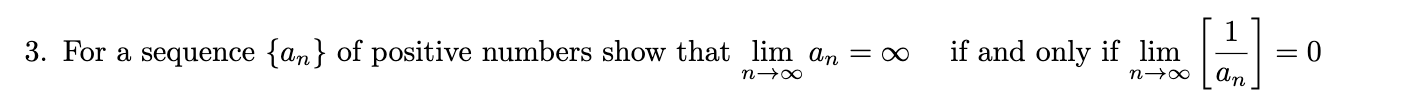
\includegraphics[width=15cm]{3.png}

\begin{proof}

  \hfill
  
$\Longrightarrow$ Suppose we are given that the sequence $\{a_n\}$ diverges such that 
$\underset{n\to\infty}{\lim}a_n = \infty$. By the definition of divergence, 
for any given $M > 0$, there exists a threshold $N \in \NN$ such that for all $n \geq N$, 
$a_n > M$. We want to show that $\frac{1}{\{a_n\}}$ converges to $0$.
\[a_n > M \ \forall n \geq N\]
where both $a_n, M > 0 \ \forall \ n$. Therefore, still for all $n \geq N$, 
\[\frac{1}{a_n} < \frac{1}{M}\]
\[-\frac{1}{M} < \frac{1}{a_n} < \frac{1}{M}\]
\[-\frac{1}{M} < \frac{1}{a_n} - 0 < \frac{1}{M}\]
\[|\frac{1}{a_n} - 0|\ < \frac{1}{M}\]
Therefore, our value of $l = 0$ as desired and our $\epsilon = \frac{1}{M}$ and there is one to one mapping from values of $M$ to 
values of $\epsilon$. Note that any $\epsilon > 0$ has a corresponding value of $M$ such that $\frac{1}{M} = \epsilon$. 
Thus, for any $\epsilon > 0$, there exists an $N$ (the same threshold used to show that $\{a_n\}$ diverges)
such that
\[|\frac{1}{a_n} - 0| < \frac{1}{M} = \epsilon \ \forall \ n \geq N \implies \lim_{n\to\infty}\frac{1}{a_n} = 0\]

\hfill

$\Longleftarrow$ The reverse direction is similar. Suppose we are given that the sequence $\{\frac{1}{a_n}\}$ converges 
to $0$. Therefore, by the definition of convergence, for any given $\epsilon > 0$, there exists a threshold 
$N \in \NN$ such that
\[|\frac{1}{a_n} - 0| < \epsilon \ \forall \ n \geq N\]
We can algebraically manipulate the above such that, while still for all $n \geq N$, 
\[-\epsilon < \frac{1}{a_n} < \epsilon\]
Note that $\frac{1}{a_n} > 0 \ \forall \ n$ is given since $a_n$ is a positive sequence. 
\[\frac{1}{a_n} < \epsilon\]
\[a_n > \frac{1}{\epsilon}\]
Let $M = \frac{1}{\epsilon}$ and once again notice the one to one correspondance. Therefore, 
for any $M > 0$, we can use the same $N$ threshold that is given to show that 
\[a_n > M = \frac{1}{\epsilon} \ \forall \ n \geq N \implies \lim_{n\to\infty}a_n = \infty\]
as desired.
\end{proof}

\newpage

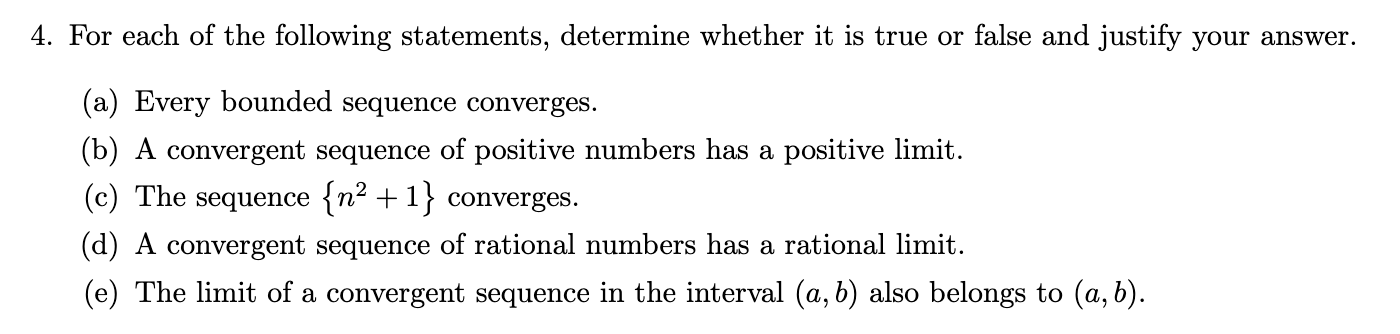
\includegraphics[width=15cm]{4.png}

\begin{enumerate}[a.]
  
\item False. Not every bounded sequence converges. For example, the sequence $\{(-1)^{n}\}$
is bounded above by $1$ and bounded below by $-1$, but it never converges.
\item False. Consider the sequence $\{\frac{1}{n}\}$ which converges to $0$, which is not positive. $0 \not> 0$.
\item False. Let $M > 0$. By A.P, $\exists \ N \in \NN$ such that $N > \sqrt{M}$. Note that $n \geq N$. Therefore, 
$n^2 + 1 \geq N^2 + 1 > M + 1 > M \implies \{n^2 + 1\}$ diverges. 
\item False. Consider a sequence such that begins as $\{3, 3.1, 3.14, 3.141, 3.14159, \cdots \}$
such that each term adds on the next digit of $\pi$. Clearly, all of these numbers are rational, as they can 
be expressed in decimal, and thus fraction, form, but the limit is $\pi \neq \QQ$. 
\item False. Consider the sequence $\{\frac{1}{n + 1}\} \ \forall \ n$. Note that $a_n \in (0, 1) \ \forall \ n$, 
yet $\underset{n\to\infty}{\lim}\frac{1}{n + 1} = 0$, and $0 \notin (0, 1)$, so this statement is false. 

\end{enumerate}

\newpage
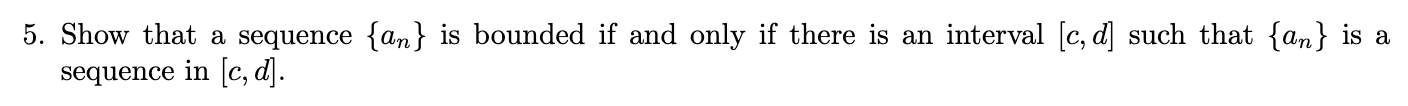
\includegraphics[width=15cm]{5.png}

\begin{proof}
  
\hfill

$\Longleftarrow$ Suppose that a sequence $\{a_n\}$ is bounded. We want to show that 
there is $[c, d]$ such that $\{a_n\}$ is a sequence in $[c, d]$. By the definition of bounded
\[\exists \ M \in \RR \text{ such that } |a_n| \leq M \ \forall \ n \in \NN\]
Therefore, for all $n$, by a property of absolute value,
\[-M \leq a_n \leq M\]
Let $c = -M$ and let $d = M$. By direct substitution, 
\[c \leq a_n \leq d\]
\[a_n \in [c, d] \ \forall \ n \in \NN\]
Thus, we've shown that there exists the interval $[c,d]$ such that $\{a_n\}$ is a sequence in $[c, d]$. 
\hfill

$\Longrightarrow$ The reverse direction is similar. Suppose that there is an interval 
$[c, d]$ such that $\{a_n\}$ is a sequence in $[c,d]$. Then we can write 
\[c \leq a_n \leq d \ \forall \ n \in \RR\]
We want to show that there exists an $M \in \RR$ such that $|a_n| \leq M \ \forall \ n$. 
Thus, let us choose $M = \max(|c|, |d|)$. This ensures that $M$ is at least greater than or equal to both 
$c$ and $d$ in terms of magnitude. We now write 
\[-M \leq c \leq a_n \leq d \leq M \ \forall \ n\]
\[-M \leq a_n \leq M \ \forall \ n\]
\[|a_n| \leq M \ \forall \ n\]
which means the sequence $\{a_n\}$ is bounded, as desired.
\end{proof}

\newpage

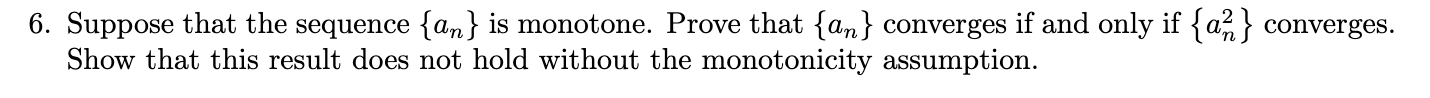
\includegraphics[width=15cm]{6.png}

\begin{proof}

\hfill

$\Longleftarrow$ Suppose the sequence $\{a_n\}$ converges. This direction is trivial because we can simply use the
Product Property. Let us denote that $\{a_n\}$ converges to $a \implies \underset{n\to\infty}{\lim}a_n = a$. 
Then by the Product Property, 
\[\lim_{n\to\infty} a_n a_n = \lim_{n\to\infty}a_n^2 = a * a = a^2 \] 
Therefore, $\{a_n^2\}$ converges to $a^2$, and so generally, it does converge, as desired.

\hfill

$\Longrightarrow$ The reverse direction is more challenging, and requires that knowledge sequence 
$\{a_n\}$ is monotone. As a counterexample without the monotonicity example, consider the sequence $\{(-1)^{2n}\}$ which converges to $1$. However, the 
square root of that sequence, $\{(-1)^n\}$ does not converge as it oscillates between $-1$ and $1$. 

\hfill

Now suppose that $\{a_n^2\}$ converges and we're given that $\{a_n\}$ is monotone.
We want to show that $\{a_n\}$ converges. Note that by a theorem, every convergent sequence 
is bounded. Therefore, $\{a_n^2\}$ is bounded. By the definition of bounded, $\exists \ M \in \RR$ 
such that 
\[|a_n^2| \leq M \ \forall \ n\]
We want to show that $\{a_n\}$ is bounded, and then we can use the Monotone Convergence Theorem to prove that the monotone sequence 
$\{a_n\}$ converges to either the $\sup, \inf$ depending on whether it is monotonically increasing
or monotonically decreasing, respectively. 
\[\sqrt{|a_n^2|} \leq \sqrt{M} \ \forall \ n\]
Note that the square operator implies that $a_n^2 \geq 0$, and so we can remove the absolute value. 
\[\sqrt{a_n^2} \leq \sqrt{M} \ \forall n\]
Now note that the square root ensures that the left hand side is greater than or equal to $0$, meaning wrapping it 
in absolute value signs will not change the result. 
\[|\sqrt{a_n^2}| \leq \sqrt{M} \ \forall n\]
\[|a_n| \leq \sqrt{M} \ \forall \ n\]
Thus, $\{a_n\}$ is bounded by $\sqrt{M} \in \RR$. Therefore, by the Monotone Convergence Theorem, 
$\{a_n\}$ converges, as desired. 
  
\end{proof}



\end{document}

